\documentclass{beamer}
\usefonttheme[onlymath]{serif}
\usepackage[T1]{fontenc}
\usepackage[utf8]{inputenc}
\usepackage[english]{babel}
\usepackage{amsmath}
\usepackage{amssymb}
\usepackage{amsthm}
\usepackage{gensymb}
\usepackage{parskip}
\usepackage{mathtools}
\usepackage{listings}
\usepackage{hyperref}
\usepackage{graphicx}
\usepackage{color}
\usepackage{enumerate}
\usepackage{tikz}
\usetikzlibrary{calc}
\usetikzlibrary{positioning}
\usetikzlibrary{angles}
\usetikzlibrary{shapes}
\usetikzlibrary{arrows}
\usepackage{verbatim}
\usepackage{multicol}
\usepackage{array}
\usepackage{minted}
\parskip 0pt


\DeclareMathOperator{\lcm}{lcm}
\newcommand\floor[1]{\left\lfloor#1\right\rfloor}
\newcommand\ceil[1]{\left\lceil#1\right\rceil}
\newcommand\abs[1]{\left|#1\right|}
\newcommand\p[1]{\left(#1\right)}
\newcommand\sqp[1]{\left[#1\right]}
\newcommand\cp[1]{\left\{#1\right\}}
\newcommand\norm[1]{\left\lVert#1\right\rVert}
\renewcommand\Im{\operatorname{Im}}
\renewcommand\Re{\operatorname{Re}}

\usetheme{metropolis}
\definecolor{dark yellow}{rgb} {0.6,0.6,0.0}
\definecolor{dark green}{rgb} {0.0,0.6,0.0}

\graphicspath{{myndir/}}

\title{Prefix Sum}
\author{Arnar Bjarni Arnarson}
\institute{\href{http://ru.is/td}{School of Computer Science} \\[2pt] \href{http://ru.is}{Reykjavík University}}
\titlegraphic{\hfill
\includegraphics[height=0.6cm]{kattis}}

\begin{document}
\maketitle

\begin{frame}[plain]{Range queries}
    \vspace{30pt}
    \begin{itemize}
        \item<1-> We have an array $A$ of size $n$.
        \item<2-> Given $i,j$, we want to answer:
            \begin{itemize}
                \item<3-> $\mathrm{max}(A[i],A[i+1],\ldots,A[j-1],A[j])$
                \item<4-> $\mathrm{min}(A[i],A[i+1],\ldots,A[j-1],A[j])$
                \item<5-> $\mathrm{sum}(A[i],A[i+1],\ldots,A[j-1],A[j])$
            \end{itemize}
        \item<6-> We want to answer these queries efficiently, or in other words, without looking through all elements.
        \item<7-> Sometimes we also want to update elements.
    \end{itemize}
\end{frame}

\begin{frame}[plain]{Range sum on constant array}
    \begin{itemize}
        \item<1-> Let's look at range sums on a constant array
        \item<2-> How do we support these queries efficiently?
    \end{itemize}

    \only<3-> {
    \begin{itemize}
        \item<3-> Simplification: only support queries of the form $\mathrm{sum}(0, j)$
        \item<4-> Notice that $\mathrm{sum}(i,j) = \mathrm{sum}(0,j) - \mathrm{sum}(0,i-1)$
    \end{itemize} }
\end{frame}

\begin{frame}[plain]{Range sum on constant array}
    \begin{itemize}
        \item<1-> So we're only interested in prefix sums
        \item<2-> But there are only $n$ of them...
        \item<3-> Just compute them all once in the beginning
    \end{itemize}
    \vspace{10pt}
    
    \only<4->{
    \begin{center}
        \begin{tabular}{|c|c|c|c|c|c|c|}
            \hline
            1 & 0 & 7 & 8 & 5 & 9 & 3 \\
            \hline
            \onslide<5->{1} & \onslide<6->{1} & \onslide<7->{8} & \onslide<8->{16} & \onslide<9->{21} & \onslide<10->{30} & \onslide<11->{33} \\
            \hline
        \end{tabular}
    \end{center} }

    \begin{itemize}
        \onslide<12->{\item $O(n)$ time to preprocess}
        \onslide<13->{\item $O(1)$ time each query}

        \vspace{10pt}
        \onslide<14->{\item Can we support updating efficiently? \onslide<15->{No, at least not without modification}}
    \end{itemize}
\end{frame}

\begin{frame}[plain]{Generalizing}
    \begin{itemize}
        \item<1-> This works on any invertible function.
        \item<2-> If we want the product we can store the products and use $\mathrm{mul}(i,j) = \mathrm{mul}(0,j) / \mathrm{mul}(0,i-1)$.
        \item<3-> This also works for multidimensional arrays, but the math is more involved.
        \item<4-> We let $\mathrm{sum}(x_i,x_j,y_i,y_j)$ denote the query for the sum from $x_i$ to $x_j$ along the $x$-dimension, and the same for $y$.
        \item<5-> Then the formula becomes
        \begin{align*}
            \mathrm{sum}(x_i,x_j,y_i,y_j) &= \mathrm{sum}(0,x_j,0,y_j) \\
                                          &- \mathrm{sum}(0,x_{i-1},0,y_j) \\
                                          &- \mathrm{sum}(0,x_j,0,y_{i-1}) \\
                                          &+ \mathrm{sum}(0,x_{i-1},0,y_{i-1})
        \end{align*}
    \end{itemize}
\end{frame}

\begin{frame}[plain]{2D sum}
    \begin{center}
        \begin{tikzpicture}
            \draw[step=1,black,thin] (0,0) grid (6,6);
            \node at (-0.1, 5.5) {\tiny \texttt{0}};
            \node at (-0.1, 4.5) {\tiny \texttt{1}};
            \node at (-0.1, 3.5) {\tiny \texttt{2}};
            \node at (-0.1, 2.5) {\tiny \texttt{3}};
            \node at (-0.1, 1.5) {\tiny \texttt{4}};
            \node at (-0.1, 0.5) {\tiny \texttt{5}};
            \node at (0.5, 6.1) {\tiny \texttt{0}};
            \node at (1.5, 6.1) {\tiny \texttt{1}};
            \node at (2.5, 6.1) {\tiny \texttt{2}};
            \node at (3.5, 6.1) {\tiny \texttt{3}};
            \node at (4.5, 6.1) {\tiny \texttt{4}};
            \node at (5.5, 6.1) {\tiny \texttt{5}};
            \node at (0.2, 6.1) {\tiny \texttt{x}};
            \node at (-0.1, 5.8) {\tiny \texttt{y}};
            \node at (8, 5.5) {\texttt{query(1, 3, 3, 4)}};
            \draw[very thick] (1, 3) -- (4, 3) -- (4, 1) -- (1, 1) -- cycle;
            \only<2-> {
                \node at (8, 4.5) {\color{blue} \texttt{query(0, 3, 0, 4)}};
            }
            \only<2> {
                \fill[blue, semitransparent] (0, 1) rectangle (4, 6);
            }
            \only<3-> {
                \node at (8, 3.5) {\color{red} \texttt{query(0, 4, 0, 2)}};
            }
            \only<3> {
                \fill[blue, semitransparent] (0, 1) rectangle (4, 3);
                \fill[red, semitransparent] (0, 3) rectangle (4, 6);
            }
            \only<4-> {
                \node at (8, 2.5) {\color{red} \texttt{query(0, 0, 0, 4)}};
            }
            \only<4> {
                \fill[blue, semitransparent] (1, 1) rectangle (4, 3);
                \fill[red, semitransparent] (0, 3) rectangle (4, 6);
                \fill[red, semitransparent] (0, 1) rectangle (1, 6);
            }
            \only<5-> {
                \node at (8, 1.5) {\color{dark green} \texttt{query(0, 0, 0, 2)}};
            }
            \only<5> {
                \fill[blue, semitransparent] (1, 1) rectangle (4, 3);
                \fill[red, semitransparent] (1, 3) rectangle (4, 6);
                \fill[red, semitransparent] (0, 1) rectangle (1, 3);
                \fill[dark green, semitransparent] (0, 3) rectangle (1, 6);
            }
        \end{tikzpicture}
    \end{center}
\end{frame}

\end{document}
